\subsection{SD-Karte}\label{sec:sdKarte}
Um auf die SD-Karte zuzugreifen, wurde die Library fatfs verwendet. Sie ermöglicht einen einfachen Zugriff auf die Daten per SPI-Schnittstelle. Sie wird im ersten Kapitel beschrieben, anschliessend behandelt ein Kapitel die Bündelung des Codes in Zusammenhang mit der SD-Karte, weshalb ein eigenes Modul geschrieben wurde. Der letzte Teil beschreibt noch die benötigten Files auf der SD-Karte, um die Funktionen des Dōjō zu gewährleisten.

\subsubsection{FatFs}
Für den Zugriff auf die SD-Karte wird ein Generic FAT Filesystem Module verwendet. In dieser Library sind Funktionen für die Initialisierung der SD-Karte und den Zugriff auf diese.

\paragraph{Lizenzen}$~~$\\
Die FatFs Library untersteht einer 1-clause BSD Lizenz. Dies bedeutet sie darf verwendet werden, muss aber den Lizenztext beiinhalten. Der Lizenztext ist im Anhang vorhanden.

\paragraph{Spezifikationen FatFs}$~~$\\
Dateisystem Typ: FAT, FAT32(rev0.0) und exFAT(rev1.0)\\
Anzahl geöffneter Dateien: unlimitiert (hängt vom verfügbaren Speicher ab)\\
Anzahl Datenträger: bis zu 10\\
Datenträgergrösse: bis zu 2TB bei 512Bytes/Sektor\\
Dateigrösse: bis zu 4GB – 1 auf FAT-Volume und praktisch unbegrenzt auf exFAT-Volume\\
Clustergrösse: Bis zu 128 Sektoren auf FAT-Volume und bis zu 16 MB auf exFAT-Volume	\\
Sektorgrösse:  512, 1024, 2048 und 4096 Bytes \cite{FatFs}\\ 

\subsubsection{SD-Karte Modul}
Nachfolgend ist beschrieben welche Funktionalitäten im Zusammenhang mit dem SD-Karten Modul vorhanden sind.

\subsubsection*{Merken}
Das Modul beinhaltet zwei Funktionen um die Funktionalität des Merken zu realisieren. Die Erste speichert das aktuelle Kunstwerk auf eine Liste. Auf dieser Liste werden die verschieden gemerkten Kunstwerken gesammelt. Die zweite Funktion löscht eben diese Liste wieder, um den Dōjō bereit für den nächsten Nutzer bereit zu machen. Den Dateinamen der Liste lässt sich im Header-File anpassen.

\subsubsection*{SD-Karte Initialisieren}
Diese Funktion ruft eine Reihe fatfs-Befehle auf um die SD-Karte zu mounten. Diese wird über ein SPI-Bus an den Microkontroller angeschlossen. Die Pins für den Bus lassen sich im Header-File definieren.

\subsubsection{Lookup}
Diese Funktion ist die eigentliche Implementierung des in Abbildung \ref{fig:lookupState} beschrieben Algorithmus.

\subsubsection*{next\_Value}
Die Funktion next Value dient dazu die nächsten Werte in den Buffer zu laden und ist wie folgt definiert:\\
\textcolor{red}{static void} next\_value(\textcolor{red}{int} bufix)\\
Sie öffnet zuerst die entsprechende Audiodatei. Dies geschieht nur zu Beginn der Datei. Sie bleibt geöffnet bis die Audiodatei zu Ende ist, oder der Benutzer das Abspielen unterbricht. Ebenfalls wird der Lesezeiger beim ersten Aufruf der Funktion auf das $44$ Byte geschoben werden, da die ersten $44$ Bytes eines WAV Files keine Audiodaten enthalten. Die Funktion liest nun 4096 Bytes in einen Hilfsbuffer ein. Die Werte werden dann daraus skaliert und in die Sequenzen geladen. Um die eine invertierte Sequenz zu erzeugen, wird das $15$ Bit auf 1 gesetzt.

\subsubsection*{Sprachwechsel}
Diese Funktion wechselt die Sprache des Dōjō. Die Sprachauswahl geschieht über verschiedene Files. Es exisitert für jede Sprache ein eigenes Lookup-File. Dieses verbindet die Majo-Minor-Kennzeichnungen mit den Wav-Files der jeweiligen Sprache. Dadurch muss für einen Sprachwechsel nur der Zeiger auf das Lookup-File geändert werden.

\subsubsection{Benötigte Files}
Im Header-File des Moduls SD-Karte müssen verschiedene Files definiert werden. Diese müssen auch auf der SD-Karte vorhanden sein und im richtigen Format. Die Merken-Liste ist eine normale Textdatei (Endung .txt). Sie sollte leer sein. Des weiteren müssen die Lookup-Files als CSV (Comma separated Value) Dateien vorhanden sein. Sie sollten dem in Abbildung \ref{fig:definition_lookup_file} definierten Format entsprechen. Zu beachten ist, dass die X Symbole für zwei stellige Hex-Zahlen stehen. Somit hat es eine Referenz auf ein Kunstwerk pro Zeile. Zu beachten ist, dass die Sprachkürzel nur zwei Zeichen beinhalten sollten.

\begin{figure}[H]
	\begin{center}
		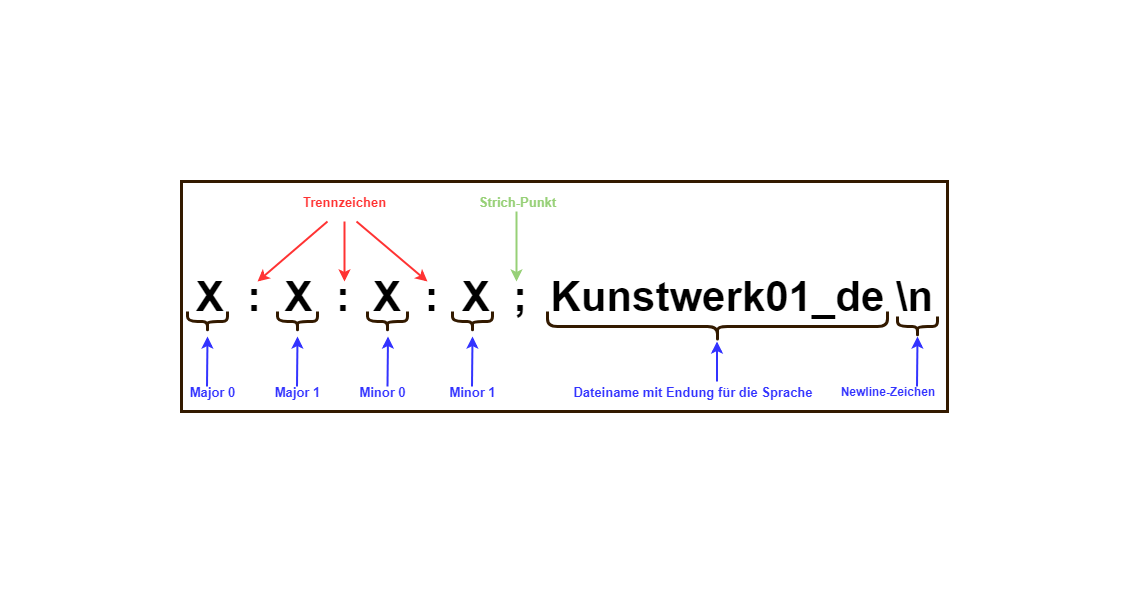
\includegraphics[width=140mm]{data/Definition_picture.png}
		\caption[Formatdefinition Lookup-File]{Formatdefinition Lookup-File} %picture caption
		\label{fig:definition_lookup_file}
	\end{center}
\end{figure}

Die Audiodateien sind im Format WAV Unsigned 8-bit PCM auf der SD-Karte abzulegen. Dabei muss beachtet werden, dass die Sample Frequenz $32 kHz$ beträgt und es sich um eine Mono-Kanal Datei handelt. 
